\section{Problem Formulation}

% --- Slide 1: How Does Pac-Man "See"? ---
\begin{frame}{How Does Pac-Man "See"? The Observation Model}
	For the neural network to make a decision, it needs a numerical representation of the game state. This is the \textbf{observation vector}.
	\vspace{1em}
	
	\textbf{Vectorial Observation Vector (26 inputs):}
	
	\begin{table}[h!]
	\centering
	\begin{tabular}{|l|l|c|}
	\hline
	\textbf{Feature} & \textbf{Description} & \textbf{\# items} \\
	\hline
	Ghost Relative Positions & $(x, y)$ for each ghost          & 8 \\
	Ghost Scared Status      & 1 bit per ghost                  & 4 \\
	Closest Dot Vector       & $(x, y)$ to nearest dot          & 2 \\
	Closest Power-up Vector  & $(x, y)$ to nearest power-up     & 2 \\
	Remaining Dots           & Number of dots left              & 1 \\
	Wall Distances           & Distance in 4 directions         & 4 \\
	Power-up Active          & 1 if power-up is active          & 1 \\
	Last Action              & One-hot, previous move           & 4 \\
	\hline
	\end{tabular}
	\caption{Total: 26 elements. \textit{Limitation: lacks spatial context.}}
	\end{table}
\end{frame}

\begin{frame}{Minimap Observation Vector (64 inputs):}
	
    The observation shown above was soon found to be ineffective. To give more awareness of the environment, I implemented an 8x8 minimap centered on Pac-Man.

    \vspace{-0.5em}

    \begin{minipage}{0.4\textwidth}
        \centering
        \vspace{0.5em}
        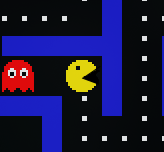
\includegraphics[width=0.8\linewidth]{assets/minimap.png}
    \end{minipage}
    \hspace{0.5em}
    \begin{minipage}{0.5\textwidth}
        \scriptsize
        $$
        \begin{bmatrix}
        \green{0.5} & \green{0.5} & \green{0.5} & 0 & 0 & \blue{-1} & \green{0.5} & 0 \\[0.5em]
        0 & 0 & 0 & 0 & 0 & \blue{-1} & \green{0.5} & 0 \\[0.5em]
        \blue{-1} & \blue{-1} & \blue{-1} & \blue{-1} & \blue{-1} & \blue{-1} & \green{0.5} & 0 \\[0.5em]
        0 & 0 & 0 & \yellow{0} & \yellow{0} & \blue{-1} & \green{0.5} & 0 \\[0.5em]
        \red{-0.75} & 0 & 0 & \yellow{0} & \yellow{0} & \blue{-1} & \green{0.5} & 0 \\[0.5em]
        \blue{-1} & \blue{-1} & \blue{-1} & \green{0.5} & 0 & \blue{-1} & \green{0.5} & 0 \\[0.5em]
        0 & 0 & \blue{-1} & \green{0.5} & \green{0.5} & \green{0.5} & \green{0.5} & \green{0.5} \\[0.5em]
        0 & 0 & \blue{-1} & \green{0.5} & 0 & 0 & \green{0.5} & 0 \\[0.5em]
        \end{bmatrix}
        $$
    \end{minipage}


    It encodes the positions of walls (\small\blue{-1}\normalsize), dots (\small\green{0.5}\normalsize), and ghosts (\small\red{-0.75}\normalsize). The four central cells represent the current Pac-Man position.

    \vspace{0.5em}

    The final observation vector is the concatenation of the vectorial observation and the minimap observation, for a total of \textbf{90 elements}.
\end{frame}

\begin{frame}{How Does Pac-Man "Learn"? The Reward Function}
	The agent's goal is to maximize its cumulative \textbf{reward}. The design of the reward function (\textit{reward shaping}) is critical to guide its behavior.
	\vspace{1em}
	
	\textbf{A naive approach is insufficient:}
	\begin{itemize}
		\item \textit{Reward only for points?} The agent might learn to get stuck in a safe corner, doing nothing.
		\item \textit{Reward only for survival?} The agent might learn to run in circles and never eat dots.
	\end{itemize}
	
	\vspace{1em}
	\textbf{The Challenge:} How do we design a task that is simple enough to be learned, yet complex enough to lead to intelligent behavior?
	
\end{frame}

\begin{frame}{Early Issues: Unintended Behaviors}
	Initial experiments with reward functions led to classic AI failures:

	\vspace{1em}
	
	\begin{columns}[T]
		\begin{column}{0.48\textwidth}
			\textbf{Reward Hacking}
			
			\vspace{0.5em}

            The agent found loopholes in the reward function. For instance:
                \begin{itemize}
                    \item If the reward function penalizes being stuck, the agent learns to oscillate between two positions.
                \end{itemize}

		\end{column}
		\begin{column}{0.48\textwidth}
			\textbf{Premature Complexity}

			\vspace{0.5em}

			\begin{itemize}
				\item Starting with the full game was overwhelming.
				\item The agent couldn't learn basic evasion while also needing to manage power-ups and complex ghost behaviors.
			\end{itemize}
		\end{column}
	\end{columns}
	
	\vspace{1em}
		These challenges motivated a structured approach: 
        \begin{center}
            \textbf{Curriculum Learning}
        \end{center}
\end{frame}